\documentclass[]{article}
\usepackage{lmodern}
\usepackage{amssymb,amsmath}
\usepackage{ifxetex,ifluatex}
\usepackage{fixltx2e} % provides \textsubscript
\ifnum 0\ifxetex 1\fi\ifluatex 1\fi=0 % if pdftex
  \usepackage[T1]{fontenc}
  \usepackage[utf8]{inputenc}
\else % if luatex or xelatex
  \ifxetex
    \usepackage{mathspec}
    \usepackage{xltxtra,xunicode}
  \else
    \usepackage{fontspec}
  \fi
  \defaultfontfeatures{Mapping=tex-text,Scale=MatchLowercase}
  \newcommand{\euro}{€}
\fi
% use upquote if available, for straight quotes in verbatim environments
\IfFileExists{upquote.sty}{\usepackage{upquote}}{}
% use microtype if available
\IfFileExists{microtype.sty}{%
\usepackage{microtype}
\UseMicrotypeSet[protrusion]{basicmath} % disable protrusion for tt fonts
}{}
\usepackage[margin=1.125in]{geometry}
\usepackage{graphicx}
\makeatletter
\def\maxwidth{\ifdim\Gin@nat@width>\linewidth\linewidth\else\Gin@nat@width\fi}
\def\maxheight{\ifdim\Gin@nat@height>\textheight\textheight\else\Gin@nat@height\fi}
\makeatother
% Scale images if necessary, so that they will not overflow the page
% margins by default, and it is still possible to overwrite the defaults
% using explicit options in \includegraphics[width, height, ...]{}
\setkeys{Gin}{width=\maxwidth,height=\maxheight,keepaspectratio}
\ifxetex
  \usepackage[setpagesize=false, % page size defined by xetex
              unicode=false, % unicode breaks when used with xetex
              xetex]{hyperref}
\else
  \usepackage[unicode=true]{hyperref}
\fi
\hypersetup{breaklinks=true,
            bookmarks=true,
            pdfauthor={},
            pdftitle={},
            colorlinks=true,
            citecolor=blue,
            urlcolor=blue,
            linkcolor=magenta,
            pdfborder={0 0 0}}
\urlstyle{same}  % don't use monospace font for urls
\setlength{\parindent}{0pt}
\setlength{\parskip}{6pt plus 2pt minus 1pt}
\setlength{\emergencystretch}{3em}  % prevent overfull lines
\setcounter{secnumdepth}{0}

\date{}

\begin{document}

\section{Serial Killer}\label{serial-killer}

\subsubsection{\texorpdfstring{\emph{a dead simple card
game}}{a dead simple card game}}\label{a-dead-simple-card-game}

\subsection{Goal}\label{goal}

Kill, kill, kill!---but don't get caught. The winner is the last serial
killer on the loose!

\subsection{Requirements}\label{requirements}

1 standard deck of playing cards\\6 counters per player (pennies,
toothpicks, etc.)

\subsection{Card summary}\label{card-summary}

\begin{itemize}
\itemsep1pt\parskip0pt\parsep0pt
\item
  \textbf{Ace} -- \emph{informant}
\item
  \textbf{King} -- \emph{victim}
\item
  \textbf{Queen} -- \emph{victim}
\item
  \textbf{Jack} -- \emph{corpse}
\item
  Numbered cards - \emph{missed opportunity!}
\end{itemize}

\subsection{Layout}\label{layout}

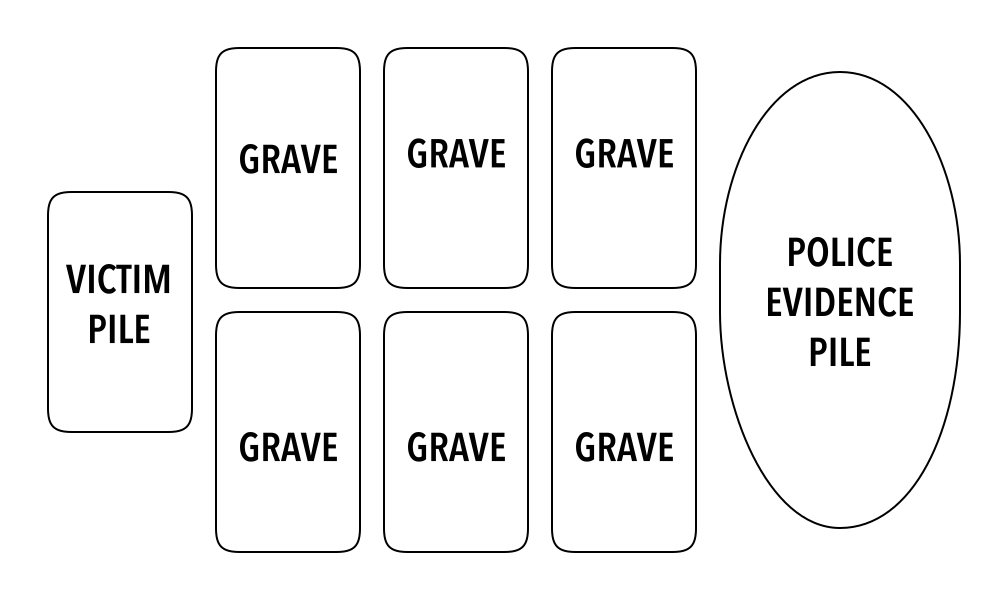
\includegraphics[width=0.8\textwidth]{img/serialkiller.png}

\subsection{Gameplay}\label{gameplay}

Each player gets 6 counters. The counters are \emph{clues}. Once the
police have all 6 of a player's \emph{clues}, they identify the player
as a serial killer, and arrested that player---the player is out of the
game. The last player with \emph{clues} left is still ``on the loose'',
and wins the game.

To select who goes first: players draw a card at random from the
shuffled deck. High card will go first. In case of a tie, players with
tied cards draw again.

To start the game: shuffle the deck. Place the deck in the ``victim
stack''.

The first player draws six cards from top of the victim stack, placing
each card into one of six ``grave'' piles. (Arrange graves so that all
players can reach them.)

Subsequent players will draw only as many cards as there are open
graves, placing each card the draw into a grave. Play proceeds
clockwise.\smallskip\hrule\smallskip

A \textbf{King} or \textbf{Queen} is a \emph{victim}.

If a player draws a \emph{victim} the player has successfully killed
that turn. When the player places the victim into a grave, that grave is
now full, and no more cards will be placed in it. Graves with numbered
cards are still open---and proof that a player missed an opportunity to
kill!

If a player does not draw a \textbf{King} or \textbf{Queen}, that player
has failed to kill that turn. The player's unsatisfied urge to kill
makes the player distracted and sloppy, and so the police find a
\emph{clue} about the player's identity.

When the police find a \emph{clue} about a player, one of that player's
counters is moved to the ``police investigation'' pile. When the police
have collected all of the \emph{clues} about a player---meaning the
player has no counters left---they arrest the player, who is then out of
the game.\smallskip\hrule\smallskip

\textbf{Jacks} and \textbf{Aces} are special cards. Players are not
required to immediately put a \textbf{Jack} or \textbf{Ace} into a
grave; they are only put into a grave when the player chooses to do so.
The player skips the grave into which the card would have been placed
when it was drawn.

Any special cards (\emph{corpses} or \emph{informants}) that a player is
holding should be kept face up and plainly visible to the other players.\smallskip\hrule\smallskip

A \textbf{Jack} is a \emph{corpse}.

Since the \textbf{Jack} is already dead, it fails to satiate a player's
need to kill, so it does not prevent the player from losing a
\emph{clue} to the police investigation pile. However, since the police
are not investigating the death of the \emph{corpse}, the player can
choose to hold onto a \emph{corpse} instead of burying it right away.

A player can use a \emph{corpse} to close a grave, by putting the
\emph{corpse} into it. A \emph{corpse} can be played at the end of any
turn of the player who drew the \textbf{Jack}.\smallskip\hrule\smallskip

An \textbf{Ace} is an \emph{informant}.

An \emph{informant} can either discredit a \emph{clue} against the
player playing the \textbf{Ace}, or can inform on another player. When
the \emph{informant} discredits a \emph{clue}, the player playing the
\textbf{Ace} gets a counter back from the police investigation pile;
when the \emph{informant} informs on another player, that player loses a
\emph{clue} to the police investigation pile.

To use an \emph{informant}, there must be a victim. If there are no
victims, the \emph{informant} cannot be played. A \emph{corpse} does not
qualify as a victim, since there is no police investigation into the
death of the \emph{corpse}.

When using an informant, the \textbf{Ace} is placed on top of a
\textbf{King} or \textbf{Queen} in a grave. A player can use an
\emph{informant} immediately when drawn, or can hold onto it. A held
\emph{informant} can be played at the end of a turn of the player who
drew the \textbf{Ace}.\smallskip\hrule\smallskip

When all six of the graves are occupied by \emph{victims} or
\emph{corpses}, reshuffle all of the unheld cards, both those in graves
and in the victim stack. Special cards---\emph{corpses} or
\emph{informants}---being held by players are not taken. The shuffled
deck is placed back in the victim stack. Play resumes where it left off.
There are once again six open graves to fill, so\ldots{}

Get out there and kill, kill, kill!

\end{document}
